\documentclass[12pt]{article}

\usepackage{amsmath, mathtools} \usepackage{amsfonts} \usepackage{amssymb}
\usepackage{graphicx} \usepackage{colortbl} % \iffalse meta-comment
%
% Copyright (C) 1993-2020
%
% The LaTeX3 Project and any individual authors listed elsewhere
% in this file.
%
% This file is part of the Standard LaTeX `Tools Bundle'.
% -------------------------------------------------------
%
% It may be distributed and/or modified under the
% conditions of the LaTeX Project Public License, either version 1.3c
% of this license or (at your option) any later version.
% The latest version of this license is in
%    https://www.latex-project.org/lppl.txt
% and version 1.3c or later is part of all distributions of LaTeX
% version 2005/12/01 or later.
%
% The list of all files belonging to the LaTeX `Tools Bundle' is
% given in the file `manifest.txt'.
%
% \fi
% \iffalse
% File: xr.dtx Copyright (C) 1993-2019 David Carlisle
%
\usepackage{xr} \usepackage{hyperref} \usepackage{longtable} \usepackage{xfrac}
\usepackage{tabularx} \usepackage{float} \usepackage{siunitx}
\usepackage{booktabs} \usepackage{caption} \usepackage{pdflscape}
\usepackage{afterpage}

\usepackage[round]{natbib}

%\usepackage{refcheck}

\hypersetup{ bookmarks=true,         % show bookmarks bar?
	colorlinks=true,       % false: boxed links; true: colored links
	linkcolor=red,          % color of internal links (change box color with
	% linkbordercolor)
	citecolor=green,        % color of links to bibliography
	filecolor=magenta,      % color of file links
	urlcolor=cyan           % color of external links
}

%% Comments

\usepackage{color}

\newif\ifcomments\commentstrue

\ifcomments
\newcommand{\authornote}[3]{\textcolor{#1}{[#3 ---#2]}}
\newcommand{\todo}[1]{\textcolor{red}{[TODO: #1]}}
\else
\newcommand{\authornote}[3]{}
\newcommand{\todo}[1]{}
\fi

\newcommand{\wss}[1]{\authornote{blue}{SS}{#1}} 
\newcommand{\plt}[1]{\authornote{magenta}{TPLT}{#1}} %For explanation of the template
\newcommand{\an}[1]{\authornote{cyan}{Author}{#1}}
 %% Common Parts

\newcommand{\progname}{SPDFM} % PUT YOUR PROGRAM NAME HERE %Every program
                                % should have a name


% For easy change of table widths
\newcommand{\colZwidth}{1.0\textwidth} \newcommand{\colAwidth}{0.13\textwidth}
\newcommand{\colBwidth}{0.82\textwidth} \newcommand{\colCwidth}{0.1\textwidth}
\newcommand{\colDwidth}{0.05\textwidth}

\newcommand{\colEwidth}{0.8\textwidth} \newcommand{\colFwidth}{0.17\textwidth}
\newcommand{\colGwidth}{0.5\textwidth} \newcommand{\colHwidth}{0.28\textwidth}

% Used so that cross-references have a meaningful prefix
\newcounter{defnum} %Definition Number
\newcommand{\dthedefnum}{GD\thedefnum} \newcommand{\dref}[1]{GD\ref{#1}}
\newcounter{datadefnum} %Datadefinition Number
\newcommand{\ddthedatadefnum}{DD\thedatadefnum}
\newcommand{\ddref}[1]{DD\ref{#1}} \newcounter{theorynum} %Theory Number
\newcommand{\tthetheorynum}{T\thetheorynum} \newcommand{\tref}[1]{T\ref{#1}}
\newcounter{tablenum} %Table Number
\newcommand{\tbthetablenum}{T\thetablenum} \newcommand{\tbref}[1]{TB\ref{#1}}
\newcounter{assumpnum} %Assumption Number
\newcommand{\atheassumpnum}{P\theassumpnum} \newcommand{\aref}[1]{A\ref{#1}}
\newcounter{goalnum} %Goal Number
\newcommand{\gthegoalnum}{P\thegoalnum} \newcommand{\gsref}[1]{GS\ref{#1}}
\newcounter{instnum} %Instance Number
\newcommand{\itheinstnum}{IM\theinstnum} \newcommand{\iref}[1]{IM\ref{#1}}
\newcounter{reqnum} %Requirement Number
\newcommand{\rthereqnum}{P\thereqnum} \newcounter{nonreqnum} %Requirement Number
% Nonfunctional
\newcommand{\rnonreqnum}{P\nonreqnum} \newcommand{\rref}[1]{R\ref{#1}}
\newcounter{lcnum} %Likely change number
\newcommand{\lthelcnum}{LC\thelcnum} \newcommand{\lcref}[1]{LC\ref{#1}}

\usepackage{fullpage}



\newtheorem{GS}{GS}





\begin{document}
	
	\title{Software Requirements Specification for\\ \progname: Surface Plasmon
		Dynamics Finite Method (SPDFM)} \author{S. Shayan Mousavi M.} \date{\today}
	
	\maketitle
	
	~\newpage
	
	\pagenumbering{roman}
	
	\tableofcontents
	
	~\newpage
	
	\section*{Revision History}
	
	\begin{tabularx}{\textwidth}{p{3cm}p{2cm}X} \toprule {\bf Date} & {\bf Version}
		& {\bf Notes}\\ \midrule 8/10/2020 & 1.0 & First Draft\\ %Date 2 & 1.1 & Notes\\
		\bottomrule \end{tabularx}
	
	~\newpage
	
	\section{Reference Material}
	
	This section records information for easy reference.
	
	\subsection{Table of Units}
	
	Throughout this document SI (Syst\`{e}me International d'Unit\'{e}s) is employed
	as the unit system.  In addition to the basic units, several derived units are
	used as described below.  For each unit, the symbol is given followed by a
	description of the unit and the SI name. ~\newline
	
	\renewcommand{\arraystretch}{1.2} %\begin{table}[ht]
	\noindent \begin{tabular}{l l l} \toprule \textbf{symbol} & \textbf{unit} &
		\textbf{SI}\\ \midrule \si{\m} & length & metre\\ \si{\per \meter} &
		reciprocal metre & wave number\\ \si{\second} & time & second\\ \si{\meter
			\per \second} & velocity & metre per second\\ \si{\kilogram} & mass	&
		kilogram\\ \si{\per \second} & frequency& hertz\\ \si{\volt \per \meter} &
		electric field strength & volt per meter\\ \si{\ampere \per \square \meter} &
		electric current density & ampere per square metre\\ \si{\farad \per \meter} &
		permittivity & farad per metre\\ \si{\henry \per \meter} & permeability &
		henry per metre\\ \bottomrule \end{tabular} %	\caption{Provide a caption}
	%\end{table}
	
	
	\subsection{Table of Symbols}
	
	The table that follows summarizes the symbols used in this document along with
	their units if applicable.
	
	\renewcommand{\arraystretch}{1.2} %\noindent \begin{tabularx}{1.0\textwidth}{l l
	% X}
	\noindent \begin{longtable*}{l l p{12cm}} \toprule \textbf{symbol} &
		\textbf{unit} & \textbf{description}\\ \midrule $\textbf{\textit{B}}$ &   &
		Basis of the Cartesian space $\in \Re^3$ \\ $\textbf{u}_x$ & & Unitary vector
		of basis \textbf{\textit{B}} $\in \Re$ \\ $\textbf{u}_y$ & & Unitary vector
		of basis \textbf{\textit{B}} $\in \Re$ \\ $\textbf{u}_z$ & & Unitary vector
		of basis \textbf{\textit{B}} $\in \Re$ \\ $\textbf{E}$ &   & 3D electric
		field vector $\in \Bbb C^3$ \\ $\textbf{E}_x$ & \si{\volt \per \meter} &
		Electric field strength along $\textbf{u}_x$  $\in \Bbb C$ \\ $\textbf{E}_y$ &
		\si{\volt \per \meter} & Electric field strength along $\textbf{u}_y$ $\in \Bbb
		C$ \\ $\textbf{E}_z$ & \si{\volt \per \meter} & Electric field strength along
		$\textbf{u}_z$ $\in \Bbb C$ \\ $\textbf{E}_i$ &   & 3D electric field vector of
		an incident light $\in \Bbb C^3$ \\ $\textbf{J}_{HD}$ &  & 3D hydrodynamic
		electric current density vector $\in \Bbb C^3$ \\ $\textbf{J}_{HD,x}$ &
		\si{\ampere \per \square \meter} & Component of hydrodynamic electric current
		density along $\textbf{u}_x$ $\in \Bbb C$ \\ $\textbf{J}_{HD,y}$ & \si{\ampere
			\per \square \meter} & Component of hydrodynamic electric current density along
		$\textbf{u}_y$ $\in \Bbb C$ \\ $\textbf{J}_{HD,z}$ & \si{\ampere \per \square
			\meter} & Component of hydrodynamic electric current density along
		$\textbf{u}_z$ $\in \Bbb C$ \\ $\varepsilon_0$ & \si{\farad \per \meter} &
		Permittivity constant $\in \Re$ \\ $\varepsilon_{loc}$ & \si{\farad \per
			\meter} & Permittivity  of the local response $\in \Bbb C$ \\ $\mu_0$ &
		\si{\henry \per \meter} & Permeability constant $\in \Re$ \\ $\nu_F$ &
		\si{\meter \per \second} & Fermi velocity $\in \Re$ \\ $\beta$ &  &Fermi
		velocity proportionality constant $\in \Re$ \\ $\omega_p$ & \si{\per \second}
		& Plasma frequency of the free electron gas $\in \Re$ \\ $\omega$ & \si{\per
			\second} & Angular frequency of the propagating wave $\in \Re$ \\ $t$ &
		\si{\second} & Time variable $\in \Re$ \\ \textbf{p} &  & Polarization vector
		of the incident light in 3D space $\in \Re^3$ \\ $p_x$ &  & Component of
		polarization vector of the incident light along $\textbf{u}_x$ $\in \Re$ \\
		$p_y$ &  & Component of polarization vector of the incident light along
		$\textbf{u}_y$ $\in \Re$ \\ $p_z$ &  & Component of polarization vector of
		the incident light along $\textbf{u}_z$ $\in \Re$ \\ \textbf{d} & & Unit
		direction vector of the incident light in 3D space $\in \Re^3$ \\ $d_x$ & &
		Component of unit direction vector of the incident light along $\textbf{u}_x$
		$\in \Re$ \\ $d_y$ & & Component of unit direction vector of the incident
		light along $\textbf{u}_y$ $\in \Re$ \\ $d_z$ & & Component of unit direction
		vector of the incident light along $\textbf{u}_z$ $\in \Re$ \\ $\lambda$ &
		\si{\meter} & Wavelength of the incident light $\in \Re$ \\ k & \si{\per
			\meter} & Wave number of the incident light $\in \Re$ \\ i & & Imaginary unit
		$\in \Bbb C$ \\ \textbf{r} &  & Displacement vector in 3D space $\in \Re$ \\
		$\varnothing()$ & \si{\meter} & Diameter operator (length of the largest
		diameter in a geometry) $\in \Re$ \\ e & & Exponential operator \\ $\nabla$ &
		& Gradient operator \\ $\times$ & & Cross product operator \\ $\textbf{.}$ & &
		Dot product operator \\ $\Omega$ & & Finite 3D meshed volume \\ $\partial
		\Omega$ & & 2D meshed boundary \\ $DtN$ & & Dirichlet to Neumann operator \\
		\bottomrule \end{longtable*}
	
	
	\subsection{Abbreviations and Acronyms}
	
	\renewcommand{\arraystretch}{1.2} \begin{tabular}{l l} \toprule \textbf{symbol}
		& \textbf{description}\\ \midrule A & Assumption\\ DD & Data Definition\\ GD &
		General Definition\\ GS & Goal Statement\\ IM & Instance Model\\ LC & Likely
		Change\\ PS & Physical System Description\\ R & Requirement\\ SRS & Software
		Requirements Specification\\ \progname{} & Surface Plasmon Dynamics Finite
		Method\\ T & Theoretical Model\\ \bottomrule \end{tabular}\\
	
	
	\newpage
	
	\pagenumbering{arabic}
	
	\section{Introduction}
	
	Surface plasmon activities are known as a bridge between the photonic realm and
	electronic physics. This material property that exist in some materials has
	opened new doors into the design of novel systems that work based on
	photon/electron interactions such as photocatalytic and optoelectronic systems.
	Therefore, it is a paramount importance to study the impact of surface plasmon
	activities on the electronic parameters in the material. This document provides
	the Software Requirements Specification (SRS) for a software designed to
	calculate the electric field and electric current density generated due to
	surface plasmon excitation in an arbitrary geometry.
	
	
	\subsection{Purpose of Document}
	
	The purpose of this document is to provide a detailed description of functional
	and the non-functional requirements of the Surface Plasmon Dynamics Finite
	Method (SPDFM) software. The theoretical models on which the requirements are
	based on are also described to provide the context of each instance model.
	
	\subsection{Scope of Requirements}
	
	The scope of requirements for the software SPDFM is limited to the realization
	of GS \ref{GS1} which measures the 3D plasmon-enhanced electric field on the
	condition that user provide sufficient environmental parameters. SPDFM is for
	the moment limited to the study of isotropic, nonmagnetic, dielectric
	environments under uniform illumination of an electromagnetic wave.
	
	\subsection{Characteristics of Intended Reader} \label{sec_IntendedReader} The
	intended reader of this work should have a minimum knowledge in mathematics and
	electrodynamics at undergraduate level. More specifically, for knowledge of
	partial differential equations, the reader can look at 
	\cite{boyce2012elementary}, for electromagnetism 
	\cite{griffiths1962introduction} is suggested, and for near-field optics the
	reader should be familiar with the concept of surface plasmons  which can be
	found in \cite{maier2007plasmonics}. Moreover, a basic knowledge in finite
	element method is recommended for deeper understanding of this document; look at
	\cite{monk2003finite}.
	
	
	\subsection{Organization of Document}
	
	The document follows the organizational scheme laid out by
	\cite{SmithAndLai2005} and  \cite{SmithEtAl2007}.
	
	
	\section{General System Description}
	
	This section provides general information about the system.  It identifies the
	interfaces between the system and its environment, describes the user
	characteristics and lists the system constraints.
	
	\subsection{System Context}
	
	Figure \ref{Fig_SystemContext} shows the system context. Circles represent the
	external entities outside the software, in this case the user and the FEniCS
	toolbox. The blue rectangle represents the \progname software system. Arrows are
	used to demonstrate the data flow between the system and the other components.
	\begin{figure}[h!] \begin{center}
			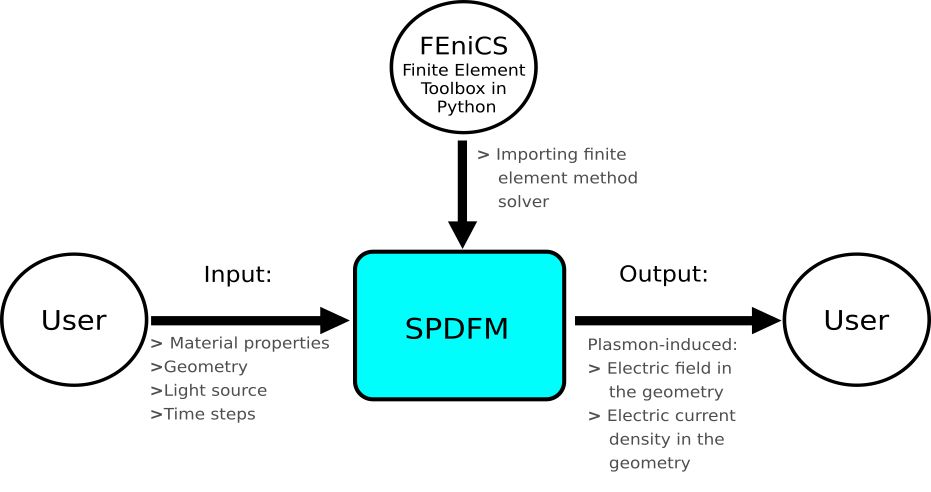
\includegraphics[width=0.6\textwidth]{SystemContextFigure.png} \caption{System
				Context} \label{Fig_SystemContext} \end{center} \end{figure}
	
	
	\begin{itemize} \item User Responsibilities: \begin{itemize} \item Provide the
			sufficient and correct data to the program. \item Be aware of impacts of user
			inputs on the quality of the output. \item Judge the correctness and accuracy of
			the data. \item Use required hardware and devices for interacting with software.
		\end{itemize}
		
		\item FEniCS toolbox Responsibilities: \begin{itemize} \item Calculate the
			solution to the provided system of equations and mesh by \progname{}.
		\end{itemize}
		
		
		\item \progname{} Responsibilities: \begin{itemize} \item Inform user of their
			responsibilities in using \progname{} \item Read input files and inform user if
			the file formats are wrong or information are missing. \item Interact with
			FEniCS toolbox. \item Display the calculated data. \item Export data in the
			correct format(s). \end{itemize} \end{itemize}
	
	\subsection{User Characteristics} \label{SecUserCharacteristics} The end user of
	\progname{} should have a relatively strong background in  Physics
	(Electromagnetism, and light/mater interaction) and Mathematics (PDEs) at
	graduate level to be able to deeply understand the data represented and properly
	utilize the software. Failing to properly interact with \progname{} has fatal
	impact on the output that can lead to some physical misinterpretations. A
	general familiarity with programming and finite element method is expected.
	
	
	
	
	\subsection{System Constraints} \progname software must be able to read .msh
	files for meshed environment import, and .csv file for the material properties
	import to be able to setup the numerical calculations system.
	
	\section{Specific System Description}
	
	This section first presents the problem description, which gives a high-level
	view of the \hyperref[Sec_pd]{problem} to be solved. This is followed by the
	solution characteristics specification, which presents the
	\hyperref[sec_assumpt]{assumptions}, \hyperref[sec_theoretical]{theories},
	\hyperref[sec_datadef]{definitions} and finally the
	\hyperref[sec_instance]{instance models}.
	
	\subsection{Problem Description} \label{Sec_pd}
	
	\progname{} is intended to calculate the 3D electric field and current density
	dynamics generated by surface plasmons in a plasmonic material.
	
	\subsubsection{Terminology and  Definitions}
	

	
	This subsection provides a list of terms that are used in the subsequent
	sections and their meaning, with the purpose of reducing ambiguity and making it
	easier to correctly understand the requirements:
	
	\begin{itemize} \item \textbf{3D Cartesian coordinate system:} An orthonormal
		system with a basis of \textbf{\textit{B}}=$\{$$\textbf{u}_x$, $\textbf{u}_y$,
		$\textbf{u}_z$$\}$ and origin of \textit{O}. For any arbitrary point in this
		space, such as \textit{R}=(x,y,z), the displacement vector \textbf{r} is: \\
		
		\begin{equation} \label{eq:planewave} \forall (x, y, z) \in \Re^3:
			\textbf{r}= x\textbf{u}_x + y\textbf{u}_y +z\textbf{u}_z \end{equation} \\
		
		\item \textbf{Mesh:} A network of coordinates in 3D Cartesian space that
		subdivides an environment or a geometry into smaller subspace. \item
		\textbf{Surface plasmon:} Collective oscillation of the free electron density on
		the surface of a conductive material due to the interaction with an
		electromagnetic of an incident photon or a swift electron beam. \item
		\textbf{Plasmonic materials:} materials such as nobel metals that have surface
		plasmonic properties.
		
		
	\end{itemize}
	
	
	\subsubsection{Physical System Description} \label{sec_phySystDescrip}

	
	
	The physical system of \progname{}, as shown in Figure \ref{fig:system},
	includes the following elements:
	
	
	\begin{itemize}
		
		\item[PS1:] An incident field (as assumed in A\ref{A_pd} is a propagating plane
		wave).
		
		\item[PS2:] $\Omega$, a 3D meshed volume (as assumed in A\ref{A_impenetrable}
		this body is impenetrable to the incident field).
		
		\item[PS3:] $\partial\Omega$, a boundary, which forms a 2D interface between
		$\Omega$ and outer environment.
		
		
		\item[PS4:] As ($\Omega$) is impenetrable, the interaction between incident beam
		and the object only takes place at the boundary which results in
		T\ref{TM:boundary}. 
	\end{itemize}
	
	
	\begin{figure}[h!] \begin{center} %\rotatebox{-90}
			{ 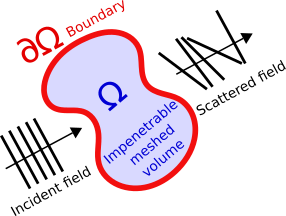
\includegraphics[width=0.5\textwidth]{physical_system.png} }
			\caption{\label{fig:system} Schematic illustration of a meshed volume
				($\Omega$) with  } \end{center} \end{figure}
	
	\subsubsection{Goal Statements} \label{goalstat} Given a meshed geometry with
	corresponding material properties (permittivity, fermi velocity, plasma
	frequency),and an incident field, the goal statement is:
	
	
	\begin{itemize}
		
		\item[GS\refstepcounter{goalnum}\thegoalnum \label{GS1}:] Calculating the
		plasmon-induced electric vector field dynamics and electric current density in
		the 3D geometry.
		
	\end{itemize}
	
	\subsection{Solution Characteristics Specification}
	
	\begin{figure}[H] 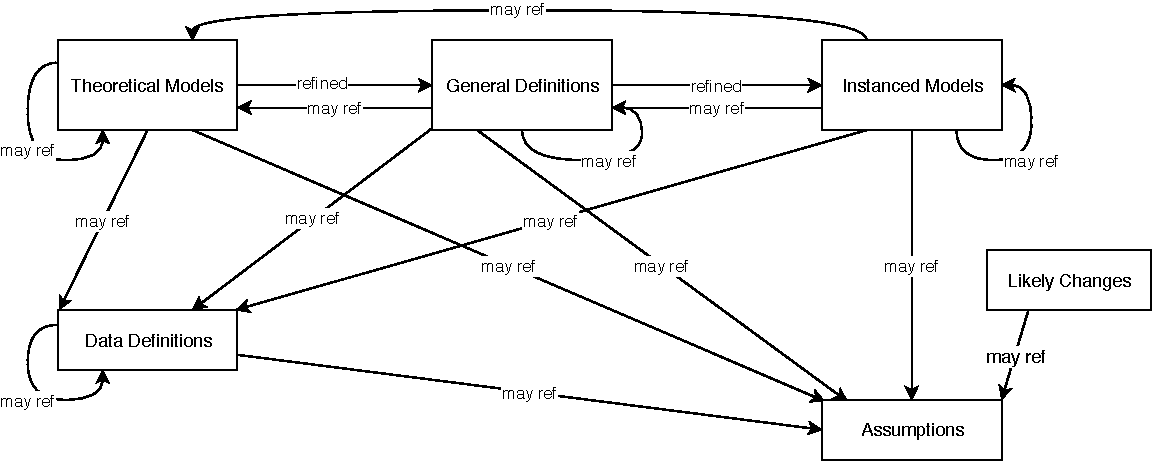
\includegraphics[scale=0.9]{RelationsBetweenTM_GD_IM_DD_A.pdf}
	\end{figure}
	
	The instance models that govern \progname{} are presented in
	Subsection~\ref{sec_instance}.  The information to understand the meaning of the
	instance models and their derivation is also presented, so that the instance
	models can be verified.
	
	\subsubsection{Assumptions} \label{sec_assumpt}
	
	
	\begin{itemize}
		
		\item[A\refstepcounter{assumpnum}\theassumpnum \label{A_nonlocal}:] Surface
		plasmon relations are governed by nonlocal hydrodynamic models and all physical
		assumptions in \cite{hiremath2012numerical} are valid.
		
		\item[A\refstepcounter{assumpnum}\theassumpnum \label{A_size}:] As \progname{}
		uses nonlocal hydrodynamic Drude physics the size of the meshed geometry is
		between 10 nm to 100 nm (\cite{hiremath2012numerical})).
		
		\item[A\refstepcounter{assumpnum}\theassumpnum \label{A_nonmag}:] The dielectric
		medium is nonmagnetic.
		
		\item[A\refstepcounter{assumpnum}\theassumpnum \label{A_pd}:] The incident field
		(light source) is a plane wave with polarization vector of \textbf{p}
		propagating towards direction \textbf{d}, therefore, $\textbf{p}.\textbf{d} =
		0$.
		
		\item[A\refstepcounter{assumpnum}\theassumpnum \label{A_wl}:] The wavelength of
		the incident field (light source) is in the range of infrared to ultraviolet.
		
		\item[A\refstepcounter{assumpnum}\theassumpnum \label{A_impenetrable}:] The
		dielectric medium is impenetrable to the incident field.
		
		\item[A\refstepcounter{assumpnum}\theassumpnum \label{A_leakage}:] Surface
		charges propagate along the surface.
		
		\item[A\refstepcounter{assumpnum}\theassumpnum \label{A_time}:] The time
		domain that surface plasmon activities are studies in the software is ranged
		from femtoseconds to microseconds.
		
		
	\end{itemize}
	
	\subsubsection{Theoretical Models}\label{sec_theoretical}
	
	This section focuses on the general equations and laws that \progname{} is based
	on. %===========T1
	
	~\newline \noindent \begin{minipage}{\textwidth}
		\renewcommand*{\arraystretch}{1.5} \begin{tabular}{| p{\colAwidth} |
				p{\colBwidth}|} \hline \rowcolor[gray]{0.9} Number&
			T\refstepcounter{theorynum}\thetheorynum \label{TM:source}\\ \hline Label&\bf
			Electric field of a propagating plane wave (light source) \\ \hline Equation&
			\begin{equation} \label{eq:planewave} \begin{gathered} \textbf{E}_{i}=
					\textbf{p}\ [ cos(k\textbf{d.r}-\omega t)- i \ sin(k\textbf{d.r}-\omega t)] \end{gathered} 
			\end{equation} \\
			
			
			\hline Description & The above equation calculates the electric field of a
			propagating plane wave (the light source) with a nonzero polarity vector $\bf
			p$, with wave number $k$ ($m^{-1}$), with unit direction vector of $\bf d$,
			and angular frequency of $\omega$ $(\si{\per \second})$. The calculated
			electric field is a 3D vector field. \\ \hline Source &
			
			\cite{monk2003finite}, section 1.3 \\ % The above web link should be
			% replaced with a proper citation to a publication
			\hline Ref.\ By & DD\ref{DD:wavenumber}, IM\ref{IM:source} \\ \hline
	\end{tabular} \end{minipage}\\
	
	%=============T2
	
	~\newline \noindent \begin{minipage}{\textwidth}
		\renewcommand*{\arraystretch}{1.5} \begin{tabular}{| p{\colAwidth} |
				p{\colBwidth}|} \hline \rowcolor[gray]{0.9} Number&
			T\refstepcounter{theorynum}\thetheorynum \label{TM:J}\\ \hline Label&\bf
			Nonlocal hydrodynamic current density (J$_{HD}$) formula \\ \hline Equation&
			\begin{equation} \label{eq:Jnonlocal} \begin{gathered}
					\dfrac{\partial^{2}}{\partial t^{2}}\textbf{J}_{HD}(\textbf{r},t)	+
					\gamma\dfrac{\partial}{\partial t}\textbf{J}_{HD}(\textbf{r},t) -
					\beta^{2}\nabla^{2}\textbf{J}_{HD}(\textbf{r},t) =
					\varepsilon_{0}\omega^{2}_{p}\dfrac{\partial}{\partial t}
					\textbf{E}(\textbf{r},t) \end{gathered}  \end{equation} \\
			
			
			\hline Description & The above partial differential equation represents the
			relationship between hydrodynamic electric current density vector
			$\textbf{J}_{HD}(\textbf{r},t)$ and electric field vector
			$\textbf{E}(\textbf{r},t)$ in time and space domain. This equation is derived
			from the definition electric current density vector and discussed in detail in
			\cite{hiremath2012numerical}. Both $\textbf{J}_{HD}(\textbf{r},t)$ and
			$\textbf{E}(\textbf{r},t)$ are in $\Bbb C^3$.\\ & In this equation $\gamma$
			(plasmon damping term (\si{\per \second}) $\in \Re$), $\beta$ (Fermi
			velocity (\si{\meter \per \second}) $\in \Re$), and $\omega_p$ (plasma
			frequency, (\si{\per \second}) $\in$ $\Re$) are material properties that
			depend on the chosen medium to study.\\ & $\varepsilon_0$ (permittivity
			constant (\si{\farad \per \meter}) $\in$ $\Re$) is a constant with value of
			$8.85418781*10^{-12}$ \si{\farad \per \meter}. \\ \hline Source &
			\cite{hiremath2012numerical} \\ % The above web link should be replaced with a
			% proper citation to a publication
			\hline Ref.\ By & GD\ref{GD:weakJ}, DD\ref{DD:beta}, IM\ref{IM:solve}\\ \hline
	\end{tabular} \end{minipage}\\
	
	~\newline
	
	%=============T3
	~\newline
	
	\noindent \begin{minipage}{\textwidth} \renewcommand*{\arraystretch}{1.5}
		\begin{tabular}{| p{\colAwidth} | p{\colBwidth}|} \hline \rowcolor[gray]{0.9}
			Number& T\refstepcounter{theorynum}\thetheorynum \label{TM:E}\\ \hline Label&\bf
			Nonlocal hydrodynamic form of curl-curl equation of electric field (\textbf{E})
			\\ \hline Equation& \begin{equation} \label{eq:Enonlocal} \begin{gathered}
					\nabla\times[\dfrac{1}{\mu_{0}}\nabla\times \textbf{E}(\textbf{r},t)] +
					\varepsilon_{0}\varepsilon_{loc}\dfrac{\partial^{2}}{\partial
						t^{2}}\textbf{E}(\textbf{r},t) = -\dfrac{\partial}{\partial
						t}\textbf{J}(\textbf{r},t) \end{gathered}  \end{equation} \\
			
			
			\hline Description & Above partial differential equation, similar to equation
			\ref{eq:Jnonlocal}, shows the relationship between \textbf{E}(\textbf{r},t)
			(electric field vector $\in \Bbb C$) and hydrodynamic electric current density
			vector $\textbf{J}_{HD}(\textbf{r},t)$. However, equation \ref{eq:Enonlocal}
			is derived from  Maxwell's equations, the approach is explained in detail in
			\cite{hiremath2012numerical}. \\ & In this equation $\mu_{0}$ (permeability
			constant with value of $1.256637062 * 10^{-6}$ \si{\henry \per \meter}) and
			$\varepsilon_{0}$ (permittivity constant with value of $8.85418781*10^{-12}$
			\si{\farad \per \meter}) are constants. \\ &$\varepsilon_{loc}$ is
			permeability of the medium ($\varepsilon_{loc}$ $\in \Bbb C$, \si{\farad \per
				\meter}). \\ \hline Source & \cite{hiremath2012numerical} \\ % The above web
			% link should be replaced with a proper citation to a publication
			\hline Ref.\ By & GD\ref{GD:weakE}, IM\ref{IM:solve}\\ \hline \end{tabular}
	\end{minipage}\\
	
	~\newline
	
	%=============T4
	~\newline
	
	\noindent \begin{minipage}{\textwidth} \renewcommand*{\arraystretch}{1.5}
		\begin{tabular}{| p{\colAwidth} | p{\colBwidth}|} \hline \rowcolor[gray]{0.9}
			Number& T\refstepcounter{theorynum}\thetheorynum \label{TM:boundary}\\ \hline
			Label&\bf General boundary condition for the nonlocal hydrodynamic system  \\
			\hline Equation& \begin{equation} \label{eq:boundary} \begin{gathered}
					\begin{cases} \int_\Omega ((\nabla \times \phi).(\mu^{-1}_{0} \nabla \times
						\textbf{E})- \omega^2\phi \epsilon_{local} \textbf{E}_i)dV + \int_{\partial
							\Omega} \phi . DtN(\textbf{E})dA\\ \ \ - i\omega \int_\Omega \phi .
						\textbf{J}_{HD}dV =  -\int_{\partial \Omega} \phi.(n \times (\mu^{-1}_0 \nabla
						\times \textbf{E}_i))dA + \int_{\partial \Omega} \phi.DtN(\textbf{E}_i)dA \\ \\
						n.\textbf{J}_{HD}=0 \ \ on \ \partial \Omega \end{cases} \end{gathered} 
			\end{equation} \\
			
			
			\hline Description & The upper equation is known as the weak formulation of
			the boundary condition on the electric field in a nonlocal hydrodynamic
			system. In this equation \textbf{n} is the unit normal vector of the surface
			of the meshed volume ($\partial \Omega boundary$), $\phi$ in an arbitrary test
			vector function in the meshed geometry ($\Omega$ domain), $\varepsilon_{loc}$
			is permeability of the medium ($\varepsilon_{loc}$ $\in \Bbb C$, \si{\farad
				\per \meter}), $\textbf{E}_i$ is the electric field of the incident light
			source, and $\omega$ ($s^{-1}$) is the angular frequency of the light source.
			\\ &$DtN$ is the Dirichlet to Neumann boundary condition which is discussed in
			detail in \cite{monk2003finite}. \\ & The lower equation is also seen in
			\ref{A_leakage} and indicates that electric current only propagates on the
			surface of the mesh geometry ($\Omega$). \\ \hline Source &
			\cite{hiremath2012numerical}, \cite{monk2003finite} \\ % The above web link
			% should be replaced with a proper citation to a publication
			\hline Ref.\ By & DD\ref{DD:omega},IM\ref{IM:solve}\\ \hline \end{tabular}
	\end{minipage}\\
	
	~\newline
	
	
	\subsubsection{General Definitions}\label{sec_gendef}
	%------------------------GD1
	~\newline \noindent \begin{minipage}{\textwidth}
		\renewcommand*{\arraystretch}{1.5} \begin{tabular}{| p{\colAwidth} |
				p{\colBwidth}|} \hline \rowcolor[gray]{0.9} Number&
			GD\refstepcounter{defnum}\thedefnum \label{GD:weakJ}\\ \hline Label &\bf Weak
			formulation of the hydrodynamic current density  \\ \hline %
			% Units&$MLt^{-3}T^0$\\
			% \hline
			SI Units& The SI unit for $|\textbf{J}|$ is \si{\ampere \per \metre}\\ \hline
			Equation& $-\int_\Omega
			\beta^2(\nabla.\psi)(\nabla.\textbf{J}_{HD})dV+\omega(\omega+i\gamma)\int_{\Omega} \psi. \textbf{J}_HD dV - i\omega \omega^2_p \int_\Omega \psi.\varepsilon_{0}\textbf{E}dV = 0 $ \\ \hline Description & The weak formulation is a notation that is adopted for the finite element methods. Derivation of above equation is discussed in \cite{hiremath2012numerical}. This equation is a different notation of equation \ref{eq:Jnonlocal} which is known as weak formulation. \\ \hline Source & \cite{hiremath2012numerical}  \\ \hline Ref.\ By & T\ref{TM:J}, IM\ref{IM:solve}, DD\ref{DD:omega}\\ \hline \end{tabular} \end{minipage}\\
	
	%----------------------------GD2
	
	~\newline
	
	\noindent \begin{minipage}{\textwidth} \renewcommand*{\arraystretch}{1.5}
		\begin{tabular}{| p{\colAwidth} | p{\colBwidth}|} \hline \rowcolor[gray]{0.9}
			Number& GD\refstepcounter{defnum}\thedefnum \label{GD:weakE}\\ \hline Label &\bf
			Weak formulation of the hydrodynamic electric field \\ \hline %
			% Units&$MLt^{-3}T^0$\\
			% \hline
			SI Units&\si{\watt\per\square\metre}\\ \hline Equation& $\int_\Omega ((\nabla
			\times \phi) . (\mu^{-1}_0 \nabla \times \textbf{E})-\omega^2
			\phi.\epsilon_{local} \textbf{E}) dV + \int_{\partial \Omega} \phi.(\textbf{n}
			\times (\mu^{-1}_0 \nabla \times \textbf{E}))dA = i\omega \int_\Omega \phi.
			\textbf{J}_{HD} dV $ \\ \hline Description & The weak formulation is a notation
			that is adopted for the finite element methods. Derivation of above equation is
			discussed in \cite{hiremath2012numerical}. This equation is a different notation
			of equation \ref{eq:Enonlocal} which is known as weak formulation. \\ \hline
			Source & Citation here \\ \hline Ref.\ By &T\ref{TM:E}, IM\ref{IM:solve},
			DD\ref{DD:omega}\\ \hline \end{tabular} \end{minipage}\\
	
	\subsubsection*{Detailed derivation of simplified rate of change of temperature}
	
	
	%---------------------------DD----------------------------
	
	\subsubsection{Data Definitions}\label{sec_datadef}
	
	\
	
	This section collects and defines all the data needed to build the instance
	models. The dimension of each quantity is also given.
	
	%-----------------------------------DD1
	
	~\newline
	
	\noindent \begin{minipage}{\textwidth} \renewcommand*{\arraystretch}{1.5}
		\begin{tabular}{| p{\colAwidth} | p{\colBwidth}|} \hline \rowcolor[gray]{0.9}
			Number& DD\refstepcounter{datadefnum}\thedatadefnum \label{DD:wavenumber}\\
			\hline Label& \bf Incident electric field wave number\\ \hline Symbol &$k$\\
			\hline % Units& $Mt^{-3}$\\
			% \hline
			SI Units & $m^{-1}$\\ \hline Equation&$k=\frac{2\pi}{\lambda}$\\ \hline
			Description & $\lambda$ is the wavelength of a given wave (m). k is Wave
			number that indicates the  number of waves (cycles) per unit distance. \\
			\hline Sources& \url{https://en.wikipedia.org/wiki/Wavenumber} \\ \hline Ref.\
			By & IM\ref{IM:source}, T\ref{TM:source} \\ \hline \end{tabular}
	\end{minipage}\\
	
	
	%-----------------------------------DD2
	
	~\newline
	
	\noindent \begin{minipage}{\textwidth} \renewcommand*{\arraystretch}{1.5}
		\begin{tabular}{| p{\colAwidth} | p{\colBwidth}|} \hline \rowcolor[gray]{0.9}
			Number& DD\refstepcounter{datadefnum}\thedatadefnum \label{DD:omega}\\ \hline
			Label& \bf Meshed geometry \\ \hline Symbol &$\Omega$ + $\partial \Omega$\\
			\hline % Units& $Mt^{-3}$\\
			% \hline
			SI Units &dimensionless\\ \hline Equation& N/A \\ \hline Description &
			$\Omega$ is the 3D set of coordinate that shape a volume together and
			$\partial \Omega$ is a set of coordinates in 3D space that form the interface
			of $\Omega$ \\ \hline Sources& N/A\\ \hline Ref.\ By & IM\ref{IM:solve},
			T\ref{TM:boundary}, GD\ref{GD:weakJ}, GD\ref{GD:weakE} \\ \hline \end{tabular}
	\end{minipage}\\
	
	~\newline
	
	%-----------------------------------DD3
	
	~\newline
	
	\noindent \begin{minipage}{\textwidth} \renewcommand*{\arraystretch}{1.5}
		\begin{tabular}{| p{\colAwidth} | p{\colBwidth}|} \hline \rowcolor[gray]{0.9}
			Number& DD\refstepcounter{datadefnum}\thedatadefnum \label{DD:beta}\\ \hline
			Label& Fermi velocity proportionality coefficient \\ \hline Symbol &$\beta$\\
			\hline % Units& dimensionless\\
			% \hline
			SI Units & $m^{-1}$\\ \hline Equation&$\beta^2 = \frac{3}{5} \nu_f^2$\\ \hline
			Description & $\nu_f$ is the Fermi velocity of electron in the medium
			($ms^{-1}$) \\ \hline Sources& \cite{hiremath2012numerical} \\ \hline Ref.\ By
			& GD\ref{GD:weakJ}, T\ref{TM:J}, IM\ref{IM:solve} \\ \hline \end{tabular}
	\end{minipage}\\
	
	~\newline
	
	%-------------------------IMs------------------------
	
	
	
	\subsubsection{Instance Models} \label{sec_instance}
	
	This section transforms the problem defined in Section~\ref{Sec_pd} into one
	which is expressed in mathematical terms. It uses concrete symbols defined in
	Section~\ref{sec_datadef} to replace the abstract symbols in the models
	identified in Sections~\ref{sec_theoretical} and~\ref{sec_gendef}.
	
	
	
	
	%----------------------Instance Model 1
	
	~\newline \noindent \begin{minipage}{\textwidth}
		\renewcommand*{\arraystretch}{1.5} \begin{tabular}{| p{\colAwidth} |
				p{\colBwidth}|} \hline \rowcolor[gray]{0.9} Number&
			IM\refstepcounter{instnum}\theinstnum \label{IM:source}\\ \hline Label& \bf
			Setting up the light source\\ \hline Input&$\textbf{p}$, $\textbf{d}$,
			$\lambda$, $\omega$ \\ & The input must satisfy: \textbf{p}.\textbf{d} = 0 \\
			\hline Output&$\textbf{E}_i$ \\ \hline Description&$\textbf{p}$ is the 3D
			polarity vector of the light source (\textbf{p}=$(p_x,p_y,p_z)$, $\textbf{p} \in
			\Re^3$).\\ &$\textbf{d}$ is the 3D unite direction vector of the propagation
			of the incident light (\textbf{d} = $(d_x,d_y,d_z)$, $\textbf{d}\in \Bbb
			R^3$).\\ &$\lambda$ is the wavelength of the light source ($\si{\meter}$).\\
			&k=$\frac{2 \pi}{\lambda}$ is the wave number of the propagating wave ($\si{\per
				\meter}$).\\ & $\omega$ is the angular frequency of the light source and can
			accept any positive value and zero ($\si{\per \second}$).\\ &$\textbf{E}_i$ is
			the 3D electric vector field calculated using Equation \ref{eq:planewave} in
			T\ref{TM:source} ($\textbf{E}_i=(E_x,E_y,E_z)$, $\textbf{E}_i\in \Bbb C^3$). \\
			\hline Sources& \cite{monk2003finite} \\ \hline Ref.\ By &  T\ref{TM:source},
			DD\ref{DD:wavenumber}\\ \hline \end{tabular} \end{minipage}\\
	
	%~\newline
	
	
	
	
	
	%--------------------------Instance Model 2
	
	~\newline \noindent \begin{minipage}{\textwidth}
		\renewcommand*{\arraystretch}{1.5} \begin{tabular}{| p{\colAwidth} |
				p{\colBwidth}|} \hline \rowcolor[gray]{0.9} Number&
			IM\refstepcounter{instnum}\theinstnum \label{IM:solve}\\ \hline Label& \bf
			Forming weak formulation of hydrodynamic equations\\ \hline Input& $\gamma$,
			$\nu_f$, $\varepsilon_0$ , $\omega_p$, $\mu_{0}$, $\varepsilon_{local}$,
			$\textbf{E}_i$, $\Omega$, $\partial \Omega$, $\Delta$t, $t_{final}$ \\ \hline
			Output&  $\textbf{J}_{HD}(\textbf{r},t)$, $\textbf{E}(\textbf{r},t)$ \\ \hline
			Description & $\gamma$ is the surface plasmon damping coefficient ($s^{-1}$).\\
			& $\beta$ is the fermi velocity ($\si{\meter \per \second}$). This material
			property is used for calculating Fermi velocity proportionality coefficient
			$\beta$ using equation \ref{eq:beta}  (\ref{DD:beta}).\\ & $\varepsilon_{0}$ is
			permittivity constant ($\si{\farad \per \meter}$). \\ & $\omega_p$ is the plasma
			frequency of the target material ($\si{\per \second}$).\\ & $\mu_{0}$ is the
			permeability constant ($\si{\henry \per \meter}$). \\ & $\varepsilon_{local}$ is
			the local permittivity ($\si{\farad \per \meter}$).
			$\textbf{E}_i$ is the electric field of the incident light in $\Bbb C$, which is obtained in IM\ref{IM:source}.
			\\ & Using above values, and
			weak form of equations T\ref{TM:J} and T\ref{TM:E}, (GD\ref{GD:weakJ} and
			GD\ref{GD:weakE}) and the boundary conditions in T\ref{TM:boundary} forms a
			system of equation that FEniCS can solve using finite element method and obtains
			the electric current density $\textbf{J}_HD(\textbf{r},t)$ and electric field
			$\textbf{E}(\textbf{r},t)$ on the meshed geometry.\\
			
			&	\begin{equation} \label{eq:FEniCS} \begin{gathered} \begin{cases}
						
						-\int_\Omega
						\beta^2(\nabla.\psi)(\nabla.\textbf{J}_{HD})dV+\omega(\omega+i\gamma)\int_{\Omega} \psi. \textbf{J}_HD dV - \\ \ i\omega \omega^2_p \int_\Omega \psi.\varepsilon_{0}\textbf{E}dV = 0 \\ \\ \int_\Omega ((\nabla \times \phi) . (\mu^{-1}_0 \nabla \times \textbf{E})-\omega^2 \phi.\epsilon_{local} \textbf{E}) dV + \\ \ \int_{\partial \Omega} \phi.(\textbf{n} \times (\mu^{-1}_0 \nabla \times \textbf{E}))dA = i\omega \int_\Omega \phi. \textbf{J}_{HD} dV
						
						\\ \\ \int_\Omega ((\nabla \times \phi).(\mu^{-1}_{0} \nabla \times
						\textbf{E})- \omega^2\phi \epsilon_{local} \textbf{E}_i)dV + \int_{\partial
							\Omega} \phi . DtN(\textbf{E})dA\\ \ \ - i\omega \int_\Omega \phi .
						\textbf{J}_{HD}dV =  -\int_{\partial \Omega} \phi.(n \times (\mu^{-1}_0
						\nabla \times \textbf{E}_i))dA + \int_{\partial \Omega}
						\phi.DtN(\textbf{E}_i)dA
						\\
						\\ n.\textbf{J}_{HD}=0 \ \ on \ \partial \Omega \end{cases} \end{gathered} 
			\end{equation} \\
			\hline Sources& \cite{hiremath2012numerical}\\ 
			\hline 
			Ref.\ By & IM\ref{IM:source}, IM\ref{IM:ampl}, T\ref{TM:E}, T\ref{TM:J}, GD\ref{GD:weakJ}, GD\ref{GD:weakE} 
			\\ \hline
	\end{tabular} \end{minipage}\\
	
	%~\newline
	
	
	~\newline
	
	
	%----------------------Instance Model 3
	
	~\newline \noindent \begin{minipage}{\textwidth}
		\renewcommand*{\arraystretch}{1.5} \begin{tabular}{| p{\colAwidth} |
				p{\colBwidth}|} \hline \rowcolor[gray]{0.9} Number&
			IM\refstepcounter{instnum}\theinstnum \label{IM:ampl}\\ \hline Label& \bf
			Finding amplitude of the fields in the domain\\ \hline Input&$\textbf{J}_{HD}(\textbf{r},t)$, $\textbf{E}(\textbf{r},t)$
			 \\
			\hline Output& $|\textbf{J}_{HD}(\textbf{r},t)|$, $|\textbf{E}(\textbf{r},t)|$
			\\
			\hline 
			Description&
			After FEniCS solving the equation system \ref{eq:FEniCS}, as $\textbf{J}_{HD}(\textbf{r},t)$, and  $\textbf{E}(\textbf{r},t)$ are in $\Bbb C$ having the magnitude of the variables are more desirable for post processing.
			 \\
			\hline Sources& \cite{monk2003finite} \\ \hline Ref.\ By &  IM\ref{IM:solve}\\ \hline \end{tabular} \end{minipage}\\
	
	~\newline
	
	

	
	
	\subsubsection{Input Data Constraints} \label{sec_DataConstraints}
	
	Table~\ref{TblInputVar} shows the data constraints on the input output
	variables.  The column for physical constraints gives the physical limitations
	on the range of values that can be taken by the variable.  The column for
	software constraints restricts the range of inputs to reasonable values.  The
	software constraints will be helpful in the design stage for picking suitable
	algorithms.  The constraints are conservative, to give the user of the model the
	flexibility to experiment with unusual situations.  The column of typical values
	is intended to provide a feel for a common scenario.  The uncertainty column
	provides an estimate of the confidence with which the physical quantities can be
	measured.  This information would be part of the input if one were performing an
	uncertainty quantification exercise.
	
	The specification parameters in Table~\ref{TblInputVar} are listed in
	Table~\ref{TblSpecParams}.
	
	\begin{table}[!h] \caption{Input Variables} \label{TblInputVar} \renewcommand{\arraystretch}{1.2} \noindent \begin{longtable*}{l l l l c} \toprule \textbf{Var} & \textbf{Physical Constraints} & \textbf{Software Constraints} & \textbf{Typical Value} & Uncertainty\\ \midrule 
			$\textbf{p}$ & $|\textbf{p}|=1,  \textbf{p} \in \Re^{3} , \textbf{p}.\textbf{d}=0$ & $|\textbf{p}|=1, \textbf{p} \in \Re^{3}, \textbf{p}.\textbf{d}=0$ & $(1,0,0)$ & N/A \\
			$\textbf{d}$ & $|\textbf{d}|=1,  \textbf{d} \in \Re^{3}, \textbf{p}.\textbf{d}=0$ & $|\textbf{d}|=1, \textbf{d} \in \Re^{3}, \textbf{p}.\textbf{d}=0$ & $(0,1,0)$& N/A\\
			$\lambda$ & $\lambda>0,  \lambda \in \Re$ & $200*10^{-9} m <\lambda<6*10^{-6} m$ & $4 * 10^{-7} m$& N/A\\	 
			$\omega$ & $\omega \geqslant 0, \omega \in \Re$ & $\omega \geqslant 0, \omega \in \Re$ & 1 THz & N/A\\ 
			$\delta t$ & $\delta t \geqslant 0, t \in \Re$ &  $t_{min} < \delta t < t_{max}$ & $10^{-14} s$ & N/A\\
			$\varnothing(\Omega)$ & $\varnothing(\Omega) > 0$ & $\varnothing(\Omega)_{\text{min}} \leq \varnothing(\Omega) \leq \varnothing(\Omega)_{\text{max}}$ & $20*10^{-9}$ \si[per-mode=symbol] {\metre} & N/A \\ 
			$t_{final}$ & $t_{final}>0$ &   $t_{min} < t_{final} < t_{max}$, $t_{final} \geqslant \delta t$ & $10^{-12} s$ & N/A\\
			 \bottomrule \end{longtable*} \end{table}

\begin{table}[!h] \caption{Specification Parameter Values} \label{TblSpecParams} \renewcommand{\arraystretch}{1.2} \noindent \begin{longtable*}{l l} \toprule \textbf{Var} & \textbf{Value} \\ \midrule $\varnothing(\Omega)_{\text{min}}$ & $10^{-8}$ \si{\metre}\\ $\varnothing(\Omega)_{\text{max}}$ & $10^{-7}$ \si{\metre}\\ $t_{min}$ & $10^{-15}$\\ $t_{max}$ & $10^{-12}$\\
		
		
		\bottomrule \end{longtable*} \end{table}

	\subsubsection{Properties of a Correct Solution} \label{sec_CorrectSolution}
	
	The correct measured variables must be judged by the user, based on him/herself
	knowledge. For simple cases user can compare the simulated result with
	analytical solutions.
	
	
	
	\section{Requirements}
	\label{req}
	
	This section provides the functional requirements, the business tasks that the
	software is expected to complete, and the nonfunctional requirements, the
	qualities that the software is expected to exhibit.
	
	\subsection{Functional Requirements}
	
	\noindent \begin{itemize}
		
		\item[R\refstepcounter{reqnum}\thereqnum \label{R_1}:] Provide user a procedure to input the environmental parameters and meshed geometry (IM\ref{IM:source}).
		
		\item[R\refstepcounter{reqnum}\thereqnum \label{R_2}:] Verify the
		format of inputs with respect to the criteria provided in table \ref{TblInputVar} (IM\ref{IM:source}).
		
		\item[R\refstepcounter{reqnum}\thereqnum \label{R_3}:] Calculate the
		electric field of the light source ($\textbf{E}_i$)
		(IM\ref{IM:source}).
		
		\item[R\refstepcounter{reqnum}\thereqnum \label{R_4}:] Calculate the
		plasmon enhance electric field and current density in the given geometry and illumination condition
		(IM\ref{IM:solve}).
	%	\item[R\refstepcounter{reqnum}\thereqnum \label{R_4}:] Verify
	%	the format of the inputs $\gamma$, $\nu_f$, $\varepsilon_0$, $\omega_p$, and
	%	$\mu_{0}$ to be scalars in $\Re$ and $\varepsilon_{local}$ to be a scalar in
	%	$\Bbb C$ (IM\ref{IM:solve}).
		
	%	\item[R\refstepcounter{reqnum}\thereqnum \label{R_5}:]Verify that all data
	%	inputs for $\Omega$ are of the correct dimensionality and composed of Real
	%	numbers (IM\ref{IM:solve}).
		
	%	\item[R\refstepcounter{reqnum}\thereqnum \label{R_6}:] Verify that all data
	%	inputs for $\Omega$ are of the correct %dimensionality and composed of Real
	%	numbers (IM\ref{IM:solve}).
		
		
		
	\end{itemize}
	
	\subsection{Nonfunctional Requirements}
	
	\begin{itemize} 
		
		\item[NR 1 \label{NR_RAM}:] The software should run on a modern
		desktop computer with a descent CPU and at least 8 GB of RAM.
		
		\item[NR 2 \label{NR_data}:] The calculated data at each step of the process
		should be accessible to the user, so that user be able monitor the evolution
		of the data.
		
		\item[NR 3 \label{NR_Output}:] The user should be able to extract the final
		data in whatever desirable format.
		
		\item[NR 3 \label{R_update}:] The software should be maintainable and
		expandable by the original programmer and future users.
		
		\item[NR 4 \label{R_compatibility}:] The software should function on any
		operating systems that can run dependant toolboxes. \end{itemize}
	
	
	\section{Likely Changes}
	
	\noindent \begin{itemize}
		
		\item[LC\refstepcounter{lcnum}\thelcnum\label{LC_lightsource}:] In the current
		version of the \progname{} plane wave propagation condition is assumed for the
		incident electric field (A\ref{A_pd}). However, as surface plasmons are
		physically damped harmonic charge oscillations, it is more accurate to study
		their dynamic after a pulse excitation when they can free damp. Therefore, it is
		possible that in future more options for the incident electric field will be
		considered such as pulsed laser illumination.
		
		\item[LC\refstepcounter{lcnum}\thelcnum\label{LC_size}:] Although \progname{} is
		formulated around nonlocal hydrodynamic responses of the electric field, by
		adding quantum formulations for smaller structures and local electrostatic
		formulations for bigger structures size of the modeled system can be more
		flexible (A\ref{A_size}).
		
		
		\item[LC\refstepcounter{lcnum}\thelcnum\label{LC_magnetism}:] Although current
		version of \progname{} is only considering nonmagnetic materials, it is likely
		to study impact of magnetism on hydrodynamic formalism and add capability of
		study these materials to the software in the future (A\ref{A_nonmag}).
		
	\end{itemize}
	
	\section{Unlikely Changes}
	
	\noindent \begin{itemize}
		
		\item[LC\refstepcounter{lcnum}\thelcnum\label{LC_wavelength}:] As this software
		is written for studying surface plasmon activities, this package will expand
		around this physical phenomenon that takes place in wavelengths ranged from
		infrared to ultraviolet (A\ref{A_wl}). Thus, it is less probable that this
		wavelength range change.
		
		\item[LC\refstepcounter{lcnum}\thelcnum\label{LC_time}:] As plasmon activities
		damp within femtoseconds, for studying these system and their interaction with
		other components in the environment time domains beyond microseconds will not
		add any useful information. Therefore changing the time domain for calculations
		in is unlikely (A\ref{A_time}).
		
	\end{itemize}
	
	\section{Traceability Matrices and Graphs}
	
	The purpose of the traceability matrices is to provide easy references on what
	has to be additionally modified if a certain component is changed.  Every time a
	component is changed, the items in the column of that component that are marked
	with an ``X'' may have to be modified as well.  Table~\ref{Table:trace} shows
	the dependencies of theoretical models, general definitions, data definitions,
	and instance models with each other. Table~\ref{Table:R_trace} shows the
	dependencies of instance models, requirements, and data constraints on each
	other. Table~\ref{Table:A_trace} shows the dependencies of theoretical models,
	general definitions, data definitions, instance models, and likely changes on
	the assumptions.
	


	
		\begin{table}[h!]
			\centering
			\begin{tabular}{|c|c|c|c|c|c|c|c|c|c|c|c|c|c|c|c|c|c|c|c|}
				\hline
				& \aref{A_nonlocal}& \aref{A_size}& \aref{A_nonmag}& \aref{A_pd}& \aref{A_wl}& \aref{A_impenetrable}& \aref{A_leakage}& \aref{A_time}\\
				\hline
				\tref{TM:source}          & & & &X &X & & &X \\ \hline
				\tref{TM:J}               &X &X &X & & & & X&  \\ \hline
				\tref{TM:E}               & X& X&X & & & & &  \\ \hline
				\tref{TM:boundary}        &X & & & & X& X& &  \\ \hline
				\dref{GD:weakJ}           & X&X & X& & & & &  \\ \hline
				\dref{GD:weakE}           & X& X& X& & & & & \\ \hline
				\ddref{DD:wavenumber}     & & & & & X& & &  \\ \hline
				\ddref{DD:omega}          & &X & & & & & &  \\ \hline
				\ddref{DD:beta}           & & & & & & & &  \\ \hline
				\iref{IM:source}          & & & &X &X & & &X  \\ \hline
				\iref{IM:solve}           &X &X &X &X & X&X &X &X  \\ \hline
				\iref{IM:ampl}       & X&X &X &X &X & X& X&X  \\ \hline
				\lcref{LC_lightsource}    & & & &X &X & & &X  \\ \hline
				\lcref{LC_size}           & X& X& & & & & &  \\ \hline
				\lcref{LC_magnetism}      & X& & X& & & & &   \\ \hline
			
				\hline
			\end{tabular}
			\caption{Traceability Matrix Showing the Connections Between Assumptions and Other Items}
			\label{Table:A_trace}
		\end{table}

\begin{table}[h!]
	\centering
	\begin{tabular}{|c|c|c|c|c|c|c|c|c|c|c|c|c|c|c|c|c|c|c|c|c|c|c|c|}
		\hline        
		& \tref{TM:source}& \tref{TM:J}& \tref{TM:E}& \tref{TM:boundary}& \dref{GD:weakJ} & \dref{GD:weakE}& \ddref{DD:wavenumber} & \ddref{DD:omega}& \ddref{DD:beta}& \iref{IM:source}& \iref{IM:solve}& \iref{IM:ampl} \\
		\hline
		\tref{TM:source}        & X& & & X& & & X& & &X &X &X \\ \hline
		\tref{TM:J}             & & X& & X& X& & & X& & & X&X \\ \hline
		\tref{TM:E}             & & & X& X& & X& & & & & X& X\\ \hline
		\tref{TM:boundary}      &X &X &X &X & & &X&X&X&X&X&X\\ \hline
		\dref{GD:weakJ}         & &X & & &X & & &X &X & &X &X \\ \hline
		\dref{GD:weakE}         & & &X & & &X & &X & & & X& X\\ \hline
		\ddref{DD:wavenumber}   & X& & & X& & & X& & &X &X &X \\ \hline
		\ddref{DD:omega}        & & & &X &X &X & &X & & &X &X \\ \hline
		\ddref{DD:beta}         & &X & & &X & & & &X & &X &X \\ \hline
		\iref{IM:source}        &X & & &X & & &X & & &X &X &X \\ \hline
		\iref{IM:solve}         &X &X &X &X &X &X &X &X &X &X &X &X  \\ \hline
		\iref{IM:ampl}          &X &X &X &X &X &X &X &X &X &X &X &X \\ 
	
		\hline
	\end{tabular}
	\caption{Traceability Matrix Showing the Connections Between Items of Different Sections}
	\label{Table:trace}
\end{table}

\begin{table}[h!]
	\centering
	\begin{tabular}{|c|c|c|c|c|c|c|c|}
		\hline
		& \iref{IM:source}& \iref{IM:solve}& \iref{IM:ampl}& \ref{sec_DataConstraints}& \rref{R_RawInputs}& \rref{R_MassInputs} \\
		\hline
		\iref{IM:source}            & & X& & & & X \\ \hline
		\iref{IM:solve}            & X& & & X& & X \\ \hline
		\iref{IM:ampl}          & & & & & & X \\ \hline
	
		\rref{R_1}     & X& & & & & \\ \hline
		\rref{R_2}     & X& & & & & \\ \hline
		\rref{R_3}     & X& & & & & \\ \hline
		\rref{R_4}     & X& & & & &  \\ \hline
		\rref{R_5}     & X& & & & &  \\ \hline 
		\rref{R_6}     & & X& & & & \\ \hline
		\rref{R_7}     & & X& & & &  \\ \hline
		\rref{R_8}     & & X& & & & \\ \hline
		\rref{R_9}     & & X& & & &  \\ \hline
		\rref{R_10}    & & X& X& & & \\ 
		\hline
	\end{tabular}
	\caption{Traceability Matrix Showing the Connections Between Requirements and Instance Models}
	\label{Table:R_trace}
\end{table}
	The purpose of the traceability graphs is also to provide easy references on
	what has to be additionally modified if a certain component is changed.  The
	arrows in the graphs represent dependencies. The component at the tail of an
	arrow is depended on by the component at the head of that arrow. Therefore, if a
	component is changed, the components that it points to should also be changed.
	Figure~\ref{Fig_ATrace} shows the dependencies of theoretical models, general
	definitions, data definitions, instance models, likely changes, and assumptions
	on each other. Figure~\ref{Fig_RTrace} shows the dependencies of instance
	models, requirements, and data constraints on each other.
	
	% \begin{figure}[h!]
	% 	\begin{center}
	% 		%\rotatebox{-90}
	% 		{
	% 			\includegraphics[width=\textwidth]{ATrace.png}
	% 		}
	% 		\caption{\label{Fig_ATrace} Traceability Matrix Showing the Connections
	% Between Items of Different Sections}
	% 	\end{center}
	% \end{figure}
	
	
	% \begin{figure}[h!]
	% 	\begin{center}
	% 		%\rotatebox{-90}
	% 		{
	% 			\includegraphics[width=0.7\textwidth]{RTrace.png}
	% 		}
	% 		\caption{\label{Fig_RTrace} Traceability Matrix Showing the Connections
	% Between Requirements, Instance Models, and Data Constraints}
	% 	\end{center}
	% \end{figure}
	
	\section{Values of Auxiliary Constants}
	
	$\varepsilon_{0} = 8.8541878128 * 10^{-12} \si{\farad\per \meter}$ \\ $\mu_{0} =
	1.256637062 * 10^{-6}$ \si{\henry \per \meter} \\
	
	\newpage
	
	\bibliographystyle {plainnat} \bibliography {../../refs/References}
	
	
\end{document}